\section{Query Implementation}
In this section, we elaborate how we have implemented the query logic to achieve O(log(n)) time complexity. The 2015 Grand Challenge problem has two queries. First is to evaluate top ten most frequent routes within last 30 minutes and second is to evaluate top ten profitable areas within last 15 minutes. We can use a composite object to keep route details for each route and fare details to each cell to compare values among routes and cells. However, each time window can have thousands of route and cell details. Therefore an efficient data structure is required to add, remove, update and retrieve top ten values from a set of objects for a given time window efficiently. Further since each event is received with route and cell details, above mentioned operations should perform using route and cell details as the key. In order to support all these functions with O(log(n)) time complexity we developed a data structure called NodeList. Following parts of this section describes how we have achieve this time complexity with \textit{NodeList} data structure and how we have implemented the queries using that data structure.

\subsection{NodeList data structure}

\begin{table}
\centering
\caption{Operations of \textit{NodeList} Data Structure}
\begin{tabular}{|l|l|} \hline
Operation Signature & Time Complexity \\ \hline \hline
add(key : Object, value : NodeValue) & O(log(n)) \\ \hline 
get(key : Object) : NodeValue & O(1) \\ \hline
remove(key : Object) : NodeValue & O(log(n)) \\ \hline
decrementPosition(key : Object) & O(log(n)) \\ \hline
incrementPosition(key : Object) & O(log(n)) \\ \hline
getTopValues() : List<NodeValue> & O(1) \\ \hline
\end{tabular}
\label{nodelist_api}
\end{table}

Table \ref{nodelist_api} shows the operations of this data structure. The NodeValue is an interface to plug any user defined type as a value. For an example, the route query can use a RouteCount object to keep route count while profitable cells query can use CellProfict object to keep fare details. This interface contains a method called compare to define the order of the values. The NodeList data structure provides the notion of a sorted values starting from position 0 (highest value) to its users. The decrementPostion operation moves the corresponding value towards position 0 until the correct position according to sorted order. Therefore this method should be called after increasing a value of an existing object. Similarly incrementPosition operation can be used to move a value to correct position after decreasing the value of an existing object. GetTopValues operation returns the top ten values of the list. Query algorithm sections further elaborate usage of these methods.

One way of implementing this data structure is to use a heap. Heap supports adding and extracting maximum value operations in O(log(n)) time. However since this application requires top 10 values, we need to retrieve maximum value ten times and insert them back, if we just a heap. On the other hand if we use a doubly linked list to keep values, it will take O(n) time for  decrementPostion and   incrementPosition operations. Therefore we can use a doubly linked list to keep first 10 values (this makes time complexity for all operations with this data structure O(1)) and heap to keep other values to avoid above problems.  A Map which points to values can be used to retrieve values using a key.

NodeList data structure uses two data structures called OrderedList to keep first 10 values and DynamicHeap to keep other values. In this way it has to change only the last value of OrderedList and maximum value of Dynamic heap as required. Following sections describes how these structures implemented with their operations.

\subsection{OrderedList data structure}

\begin{table}
\centering
\caption{Operations of \textit{OrderedList} Data Structure}
\begin{tabular}{|l|l|} \hline
Operation Signature & Time Complexity \\ \hline \hline
add(key : Object, value : NodeValue) & O(n) \\ \hline
containsKey(key : Object) : boolean & O(1) \\ \hline
get(key : Object) : NodeValue & O(1) \\ \hline
incrementPosition(key : Object) & O(n) \\ \hline
decrementPosition(key : Object) & O(n) \\ \hline
remove(key : Object) : NodeValue & O(1) \\ \hline
getLastPosition() : int & O(1) \\ \hline
getLastKey() : Object & O(1) \\ \hline
\end{tabular}
\label{orderedlist_api}
\end{table}

Table \ref{orderedlist_api} shows the operations of the \textit{OrderedList} data structure. First six methods has the same meanings as the \textit{NodeList} data structure and last two can be used to get the size of the list and the value of the last object. We internally keep a counter and a pointer to tail to support these operations in O(1) time. Figure \ref{orderedlist_impl} shows the implementation details. The Map structure (an HashMap) is used to retrieve object pointers with O(1) expected time. Each node of the doubly linked list points to previous and next nodes while storing the \textit{NodeValue}.


\begin{figure}[!t]
        \centering
        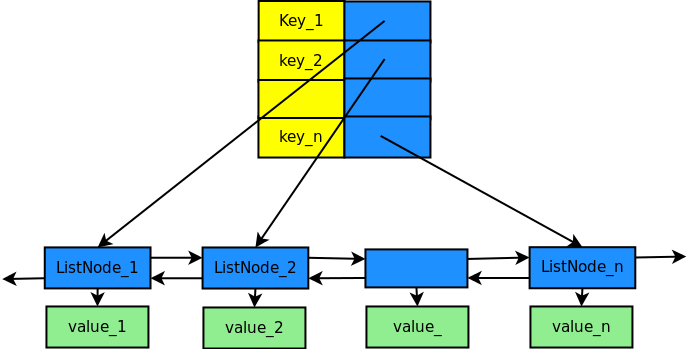
\includegraphics[width=3.0in]{orderedlist.png}
        \caption{\textit{OrderedList} data structure implementation}
        \label{orderedlist_impl}
\end{figure}

\subsection{DynamicHeap data structure}

\begin{table}
\centering
\caption{Operations of \textit{DynamicHeap} Data Structure}
\begin{tabular}{|l|l|} \hline
Operation Signature & Time Complexity \\ \hline \hline
add(key : Object, value : NodeValue) & O(log(n)) \\ \hline
remove(key : Object) : NodeValue & O(log(n)) \\ \hline
containsKey(key : Object) : boolean & O(1) \\ \hline
get(key : Object) : NodeValue & O(1) \\ \hline
moveUp(key : Object) & O(log(n)) \\ \hline
moveDown(key : Object) & O(log(n)) \\ \hline
getMaxkey() : Object & O(1) \\ \hline
extractMax() : NodeValue & O(log(n)) \\ \hline
\end{tabular}
\label{dynamicheap_api}
\end{table}

Table \ref{dynamicheap_api} shows the operations of the \textit{DynamicHeap} data structure. \texttt{MoveUp} and \texttt{moveDown} operations are used to move an element up in the heap if the value increased, or move down in the heap if the value decreased. Figure \ref{dynamicheap_impl} shows the implementation details. Conventional heaps only support \texttt{add} and \texttt{extractMax} operations since heap operations requires to know the element position in heap. When adding an element we add it to last position and move that up and extracting maximum element start at array position 0. In order to support \texttt{moveUp}, \texttt{moveDown} and \texttt{remove} operations, we keep the array index with the object itself. This allows us to retrieve array index in O(1) time and move the element O(log(n)) time.


\begin{figure}[!t]
        \centering
        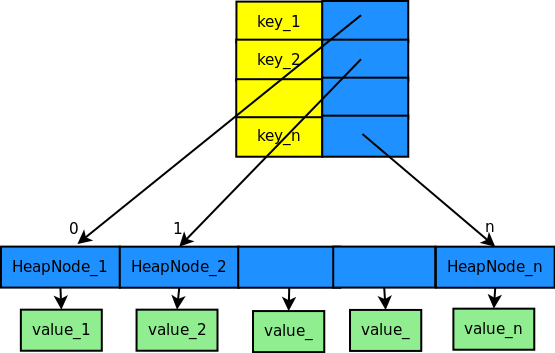
\includegraphics[width=3.0in]{DinamicHeap.png}
        \caption{\textit{DynamicHeap} data structure implementation}
        \label{dynamicheap_impl}
\end{figure}

\subsection{Frequent Route Query}

Frequent route query requires to find the top frequent routes within last 30 minutes. Algorithm \ref{frequent_route_algorithm} shows the algorithm to process this query using the \textit{NodeList} data structure and a queue to keep the events for the time window.  Since queue operations are supported in O(1) time, query evaluation happens in O(log(n)) time. Algorithm \ref{frequent_route_algorithm} shows the basic algorithm to process an event. This algorithm assumes there is a global NodeList object and route counts stored in an Object called RouteCount. 

\begin{algorithm}
\caption{Algorithm to generate top 10 frequent route change events}
\label{frequent_route_algorithm}
\begin{algorithmic} 
\STATE beforeTopTen $\leftarrow$ nodeList.getTopValues() 
\STATE window.add(event) 
\IF{ nodeList.containsKey(event.route) }
	\STATE routCount $\leftarrow$ nodeList.get(event.route) 
	\STATE routCount.count++ 
	\STATE nodeList.decrementPosition(event.route) 
\ELSE
	\STATE nodeList.add(event.route, new RouteCount(1)) 
\ENDIF

\WHILE{ there exists expired events }
	\STATE  expEvent $\leftarrow$ window.poll() 
	\STATE  routCount $\leftarrow$ nodeList.get(expEvent.route)
	\STATE  routCount.count-- 
	\IF{ routCount.count is 0 }
		\STATE nodelist.remove(expEvent.route)
	\ELSE
		\STATE nodeList.incrementPosition(expEvent.route) 
	\ENDIF
\ENDWHILE

\STATE nowTopTen $\leftarrow$ nodeList.getTopValues() 

\IF{ preTopTen not equals nowTopTen }
	\STATE create new event with top ten route details 
\ENDIF

\end{algorithmic}
\end{algorithm}

Processing an event can cause add, remove or update values of the existing time window objects. Therefore query processing mainly involves with performing above operations to the underlying \textit{NodeList} data structure and compare before and after top ten routes. As shown in Algorithm \ref{frequent_route_algorithm}, when an event arrives, first it put the event to time window to keep track for last 30 minutes. Then it adds new route value or update the existing value and move its position. Similarly, for expired events either it removes the values or reduces the count for existing values. Finally, two lists are compared to decide whether to generate an event or not. Here we have given a rough out line of the algorithm. Real implementation considers other factors such as sequence number to order events.

\subsection{Profitable Cells Query}

We have implemented profitable cells query in a similar manner to the frequent route query using  time windows. Complexity of the query raised following issues and we have solved them as given bellow.
\begin{enumerate}
	\item The profitability is calculated using the median profit and the number of empty taxis. In order to calculate median with O(log(n)) time complexity, we use two heaps (java.util.PriorityQueue) . One is used to keep the values lesser than the median value (max heap) and other is to keep higher values (min heap). However the delete operation of java.util.PriorityQueue takes O(n) time, since it traverse along the array to find the index of the object. We tried with our DynamicHeap implementation to fix this. But that did not improved the performance. Firstly, these heap sizes does not grow over the value of 60 and there are same values repeating in the list increasing the probability of find a value without traversing the whole list. Secondly, our implementation create more objects compared to just keeping double values though the time complexity is O(log(n)). 
	\item In order to keep tract of empty taxis, we need to process both pickup cell and drop off cell details for each message. One way of doing this is to send all events for same process instance and process both details with one event. However this avoid the possibility of partitioning data across different processes. We generate two events one for pickup data and one for drop off data to make the process parallel. 
	\item In order to handle expiration of drop off events, we keep track of the taxi ids currently available in a particular cell. If a pickup event occurs before drop off event expiration, then we remove that taxi id from that cell and reduce the empty taxi count. In such a case drop off event expiration does not cause a reduction of taxi count.
\end{enumerate}






